\documentclass[conference,10pt]{IEEEtran}
\usepackage{fancyhdr}
\usepackage{amssymb}
\usepackage{amsmath}
\usepackage{amsfonts}
\usepackage[T1]{fontenc} % get tt fonts to work right
\usepackage{graphicx}
\usepackage{fixltx2e}
\usepackage{multirow}
\usepackage{color}
\usepackage{caption}
\DeclareCaptionType{copyrightbox} % workaround for bug in caption
\usepackage{subcaption}
\usepackage{xspace}
\usepackage{url}

\begin{document}

\special{papersize=8.5in,11in}
\setlength{\pdfpageheight}{\paperheight}
\setlength{\pdfpagewidth}{\paperwidth}


\title{Mapping HALO Exchange onto Toruses and Stuff}

\author{\IEEEauthorblockN{
Yadu Nand\IEEEauthorrefmark{1}\IEEEauthorrefmark{2}\IEEEauthorrefmark{3},
Timothy G. Armstrong\IEEEauthorrefmark{1}}
  \IEEEauthorblockA{
  \IEEEauthorrefmark{1}Dept. of Computer Science,
    University of Chicago,
    Chicago, IL, USA}
  \IEEEauthorblockA{\IEEEauthorrefmark{2}Mathematics and Computer Science Division,
    Argonne National Laboratory,
    Argonne, IL, USA}
  \IEEEauthorblockA{\IEEEauthorrefmark{3}Computation Institute,
    University of Chicago and Argonne National Laboratory,
    Chicago, IL, USA}
}

\maketitle


\begin{abstract}
Abstract != Introduction.
[TODO]
\end{abstract}

\section{Introduction}

% Intro
Halo exchange is a common communication pattern in parallel codes, where
each process is assigned an application subdomain and must periodically
communicate with other processors that have neighboring subdomains to
update information about the state of the boundary between subdomains.
A common special case is when a multi-dimensional cartesian space is
decomposed into subdomains of equal size.  For example, in the three-dimensional
case, a 8x8x8 cube might be decomposed into 256 2x1x1 cubes for execution on 256 processors.

This paper explores the problem of mapping such multi-dimensional cartesian
halo exchange communications onto parallel computers with hypercube or
torus networks.

% Objective


% Justification
% Background
% Guidance
% Summary conclusions

\section{High-Performance Computer Networks}

The state of the art in High Performance Computing(HPC) infrastructure, demands high-performance networks
to support the movement of data between the nodes as well as to-and-from disk-arrays. HPC systems are
increasingly architected with high radix interconnects such as hypercubes and N-dimensional tori.
Parallel applications have a wide range of task placements options to exploit the network topology of
these HPC systems. These networks have evolved to several different network topologies in order to support
different requirements, and data movement patterns. For HPC applications which involve fine-grained communication,
high-radix networks provide low latency, smaller diameter, and large bandwidth as multiple links along the multiple
dimensions supprted.

% Routing protocols on the BG/Q
% Direct routing
% Adaptive routing

We are using Message Passing Interface (MPI) to implement the messaging and synchronization aspects of the HALO exchange code,
and hence the performance observed from running the application would be influenced by the behavior of MPI due to it's
various protocols on the BlueGene/Q. There are four protocols supported by the MPI implementation used BlueGene/Q.
The protocol utilized by MPI is determined by the size of the message that is being sent. The data sizes at which the switch to
different protocol occurs is configurable, but for our experiments we are using the defaults on BlueGene/Q. 

\begin{center}
    \begin{tabular}{ | l | l | l | p{2cm} |}
    \hline
    Protocol   & Min Data Limit & Max Data Limit & Routing \\ \hline
    Immediate  &              0 &            112 & Direct\\ \hline
    Short      &            113 &            496 & Direct\\ \hline
    Eager      &            497 &           2048 & Direct\\ \hline
    Rendezvous &           2048 &      unlimited & Adaptive\\ \hline
    \hline
    \end{tabular}
\end{center}

We're going to cite Swift/T~\cite{SwiftT_2013} and include an illustration
(see Figure~\ref{fig:task-data}).

\label{sect:ddt-model}
\begin{figure}
  \center
  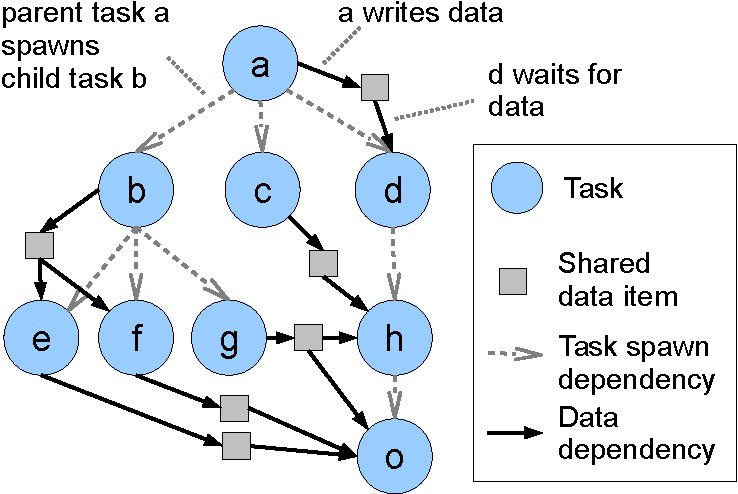
\includegraphics[width=0.325\textwidth]{fig/task-data}
  \caption{This is a figure.
    \label{fig:task-data}}
\end{figure}


\label{sect:Analytic-model}
\begin{figure}
  \center
  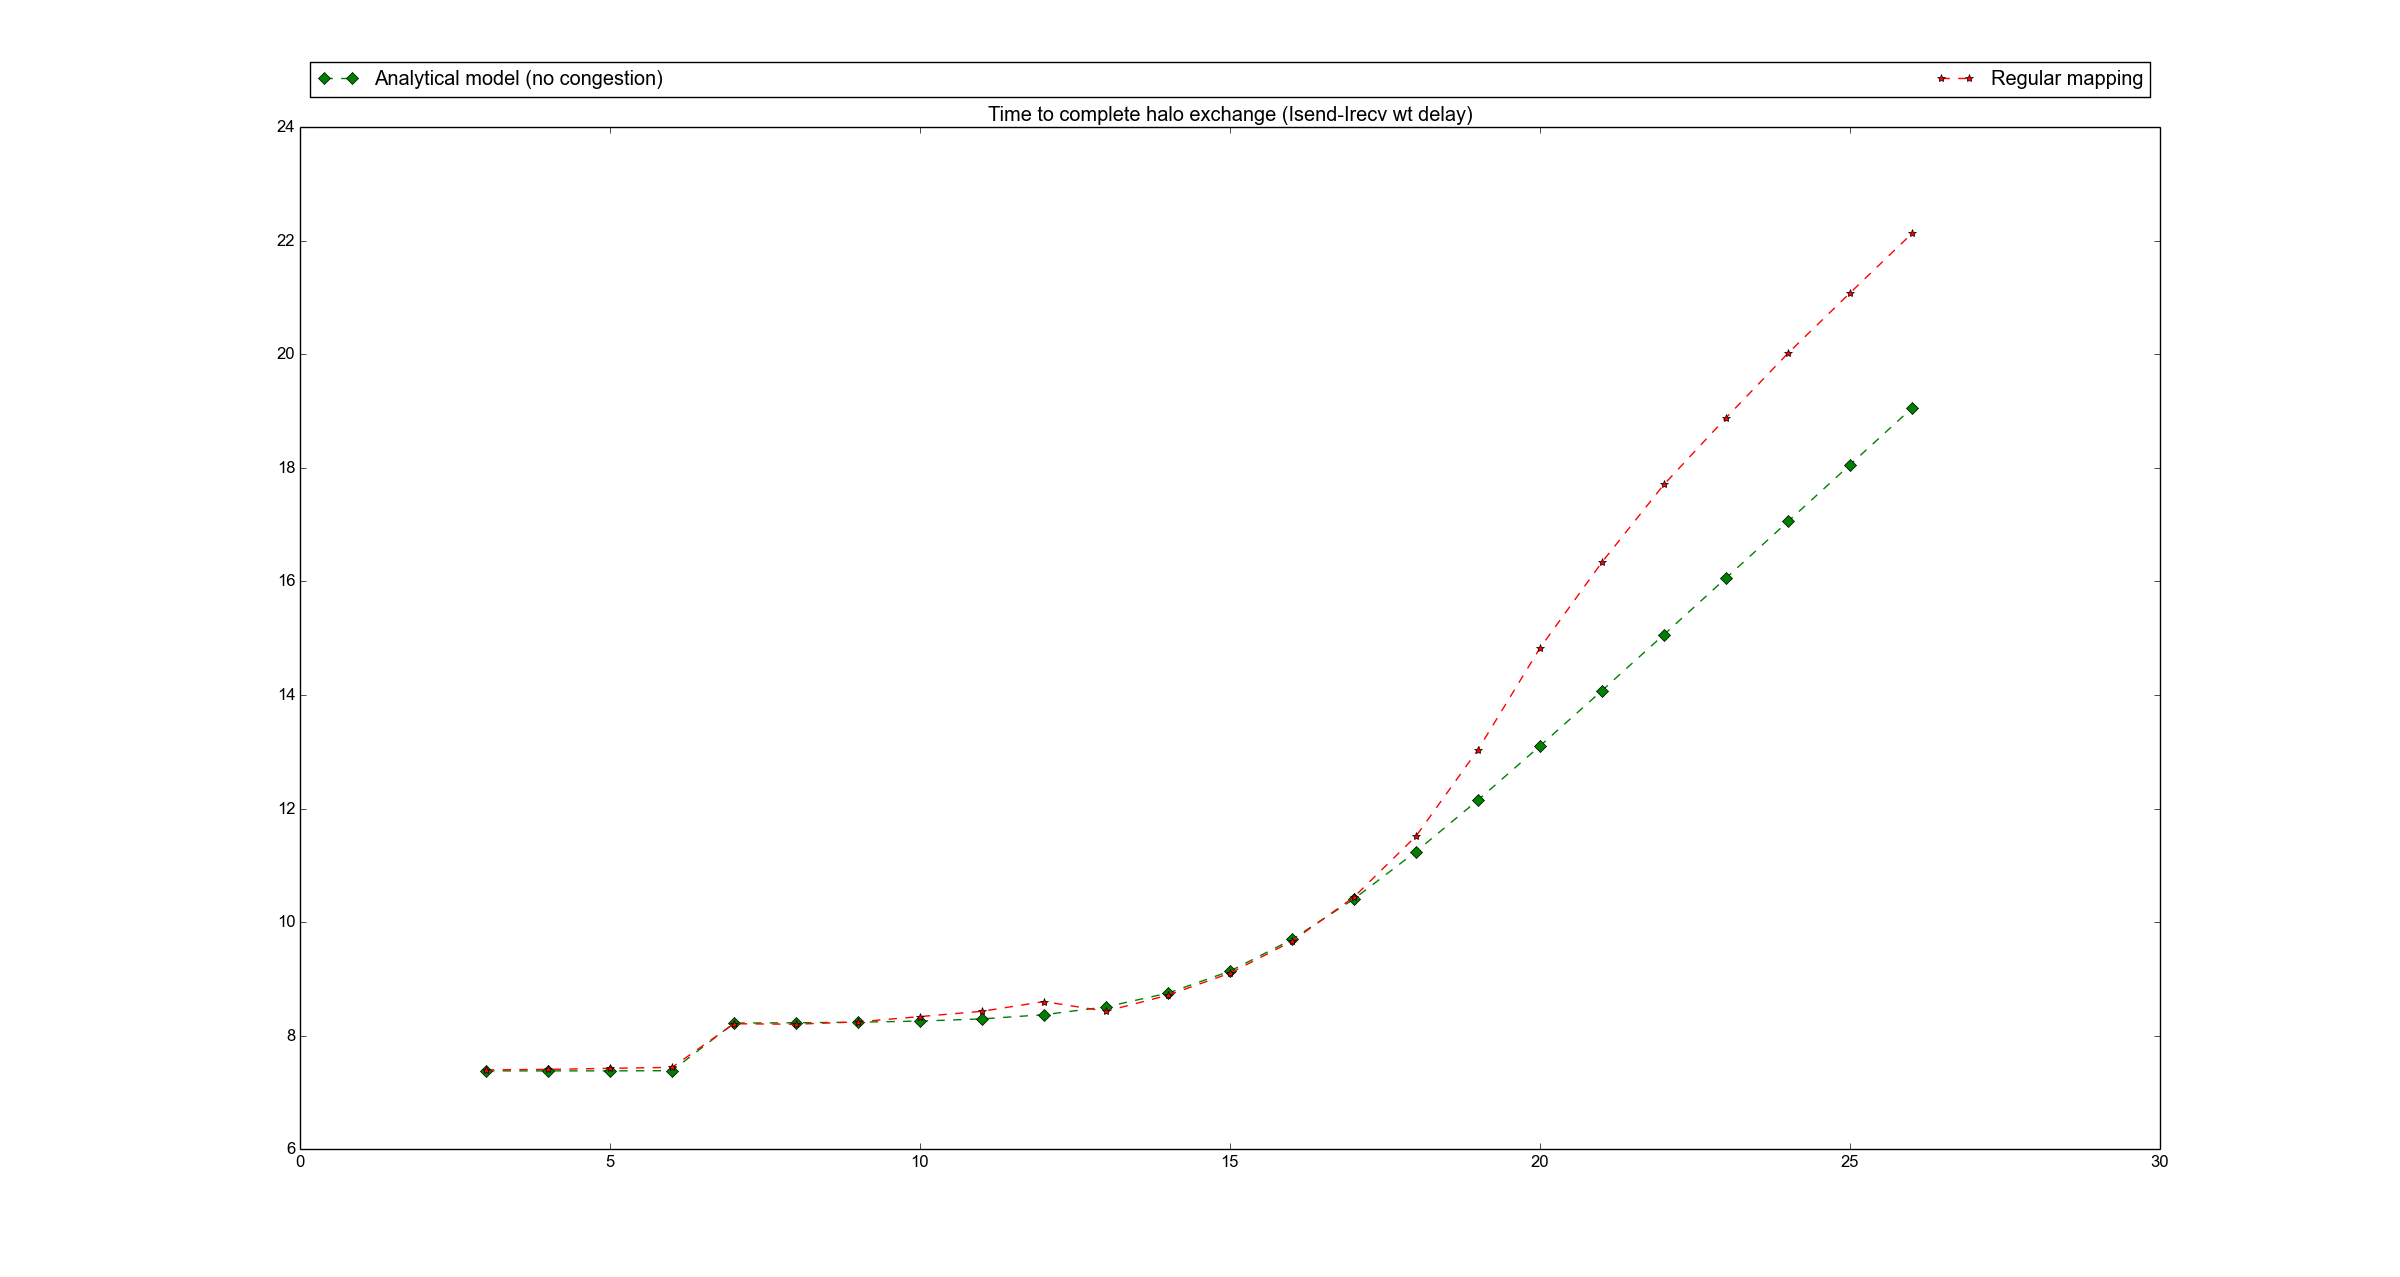
\includegraphics[width=0.325\textwidth]{fig/Analytic_regular_no_congestion_170_304_304.png}
  \caption{This is a figure.
    \label{fig:Analytic_regular_no_congestion_170_304_304.png}}
\end{figure}

\section{High-Performance Computer Networks}

\subsection{Blue Gene/Q 5D torus}
RedBook~\cite{BGQ_RedBook_2013}

\subsection{Cray Gemini 3D torus}

\section{Models for Network Communication}

On an HPC system such as BlueGene/Q or Cray XE6, each node has multiple duplex links to it's neighbors.
If the application on every node attempts to exchange messages with every neighbor, we can assume that
every link on the network will see similar traffic. Thus we, consider a single link and it's bandwidth
to determine t\textsubscript{b} the time required to send a Byte along the link. Assume that there are N\textsubscript{procs} number
of identical processes all of which will attempt to utilize the same links. To capture the differences
between different mappings we use a simple program to calculare the average distance between neighbors,
N\textsubscript{steps}. The current MPI implementation on leadership class systems like Mira (Bluegene/Q) utilizes
shared memory for intranode communication. When a neighbor is present within the same node, the link
is weighted as zero, and every network link or hop is weighted as one. Since it is possible to place
neighboring tasks from the application domain on the same node there are mappings possible which
minimize N\textsubscript{steps} below one. There are constant costs involved in startup, acquiring a buffer etc,
and t\textsubscript{c} is an experimentally calibrated constant that is a catch-all for the various constant costs
of network communication using MPI. N is the message size in bytes that are exchanged between neighbors.

A simple analytical model determines the time to completion, T of a complete halo exchange operation,
from the variables defined above as follows:

\begin{equation}
  T = t_c + (N_{steps} * N_{procs} * N * t_b)
\end{equation}

Since we have a complex set of operations on several hundreds of nodes, there is a cost for synchonisation.
We use MPI barriers to synchronise all tasks before and after measurements

\section{Experimental Design}

\section{Results}

\section{Conclusion}


\bibliographystyle{abbrv}
\bibliography{halo}

\end{document}
